\chapter{Opis projektnog zadatka}
		
	
		\textnormal{Ideja ovog projekta je napraviti web aplikaciju za košarkaški klub Rudeš. Navedeni klub trenutno ima svoje web stranice, međutim izrađene su korištenjem vrlo jednostavnog programa (WYSIWYG Web Builder) kojim se web stranicu izrađuje najobičnijom drag ‘n’ drop metodom. Zbog toga trenutna web stranica nema nikakav backend niti bazu podataka tj. nikakve karakteristike nečega što bismo nazvali pravom web aplikacijom. Link na trenutnu stranicu jest https://www.kkrudes.com.
		}
	
		\textnormal{Cilj ovog projekta je to promijeniti i čitav site napraviti ponovno, ni iz čega, ali s jasno istaknutim funkcionalnostima koje su potrebne klubu.
		Prilikom pokretanja aplikacije vidljiva je početna stranica kluba gdje se nudi mogućnost prijave u sustav. Korisnik se može prijaviti postojećim računom, za koji je potreban e-mail i lozinka, ili registrirati novim računom. Ukoliko korisnik nije registriran, može pregledavati sadržaj web stranice, što uključuje pregled igrača, utakmica, kontakta kluba i novosti vezanih uz klub. Neregistrirani korisnik također može pretraživati webshop i dodavati artikle u košaricu, ali ne može obaviti kupovinu. Za registraciju korisnika potrebno je sljedeće: }
	\begin{packed_item}
		\item korisničko ime
		\item lozinka
		\item e-mail adresa
		\item ime
		\item prezime
	\end{packed_item}
   \textnormal{ Za prijavu u sustav nije potreban broj kartice niti broj mobilnog telefona, no može se dodati prilikom kupnje u webshopu. Korisnik koji je registriran može mijenjati svoj račun ili ga obrisati. Neregistrirani korisnik registracijom postaje klijent.}
\bigbreak
\underline{\textit{Klijent} }\textnormal {je korisnik koji osim što ima sve ovlasti kao i neregistrirani korisnik, dodatno može gledati prijenos utakmica uživo i obaviti kupovinu u webshopu. Klub posjeduje svoje hoodice, majice i dresove koji se mogu naručiti tj. kupiti.
Klijent u webshopu stavlja u košaricu artikle koje želi kupiti i ukoliko se odluči na kupnju, prosljeđuje ga se do plaćanja gdje se transakcija izvrši i obavijesti upravu. 
Klijent u webshopu može ocjenjivati artikle, birati veličine i dodavati te mijenjati informacije o plaćanju kreditnom karticom. Također, može uključiti obavijesti da mu se na e-mail kojim se registrirao šalju novosti o novodostupnim artiklima i popustima u webshopu. Kako KK Rudeš ponekad prenosi svoje utakmice uživo na YouTubeu, aplikacija bi nudila dio rezerviran za streaming koji je povezan s YouTubeom i omogućuje prijavljenim korisnicima gledanje utakmica uživo, tj. prijenosa. S desne strane prijenosa nalazi se prilagođeni chat u kojem korisnici mogu komunicirati za vrijeme prijenosa. Dok nema prijenosa, u dijelu rezerviranom za prijenose pišu informacije o idućoj utakmici ili prijenosu, što je poznato unaprijed.}
\bigbreak
\textnormal {Među registriranim korisnicima postoje još 2 tipa korisnika, a to su administrator aplikacije te treneri, odnosno uprava kluba.}
\bigbreak
\underline{\textit{Treneri kluba} }\textnormal {su zaduženi za kreiranje sadržaja web aplikacije. U sadržaj ubrajamo slike, novosti te podatke kluba.  Također imaju ovlasti upravljanja igračima, odnosno mogu mijenjati njihove podatke.}
\bigbreak
\underline{\textit{Uprava kluba, tj. članovi uprave}} \textnormal {imaju ovlasti za dodavanje i mijenjanje artikla u webshopu. Imaju na uvid koliko je veličina pojedinih artikala ostalo te ih mogu dodavati, mijenjati cijene, dodavati popuste ili brisati.}
\bigbreak
\textit{\underline{Administrator  aplikacije} }\textnormal {je korisnik s najvećim ovlastima. On ima potpuni pristup bazi podataka i može brisati i dodavati trenere. Ima sve ovlasti kao i treneri/uprava kluba, s dodatkom da može nekoga od trenera ili uprave proglasiti administratorom. Može i brisati recenzije koje nisu u skladu s pravilima aplikacije.}
\bigbreak
\textnormal{Aplikacija je lokalizirana na hrvatski i engleski jezik. Sustav podržava rad više korisnika u stvarnom vremenu.}
\textnormal{Stranica će biti javno objavljena te će ju moći koristiti bilo tko s pristupom internetu. Korist ovog projekta je u tome da će stranicu koristiti sadašnji i budući članovi KKRudeš. Jedna od mogućih nadogradnji jest lokaliziranje aplikacije na njemački jezik te dodavanje foruma za raspravu o košarkaškim, a i ostalim temama širokog spektra.}
		
		


		
		\section{Primjeri u LaTeXu}
		
		\textit{Ovo potpoglavlje izbrisati.}\\

		U nastavku se nalaze različiti primjeri kako koristiti osnovne funkcionalnosti LaTeXa koje su potrebne za izradu dokumentacije. Za dodatnu pomoć obratiti se asistentu na projektu ili potražiti upute na sljedećim web sjedištima:
		\begin{itemize}
			\item Upute za izradu diplomskog rada u LaTeXu - \url{https://www.fer.unizg.hr/_download/repository/LaTeX-upute.pdf}
			\item LaTeX projekt - \url{https://www.latex-project.org/help/}
			\item StackExchange za Tex - \url{https://tex.stackexchange.com/}\\
		
		\end{itemize} 	


		
		%Ovo poglavlje je potrebno prilikom predaje obrisati
		
		\underbar{podcrtani tekst}, 
		\textbf{podebljani tekst}, 
		\textit{nagnuti tekst}\\
		\normalsize primjer
		\large primjer
		\Large primjer
		\LARGE {primjer}
		\huge {primjer}
		\Huge primjer
		\normalsize
				
		\begin{packed_item}
			
			\item  primjer
			\item  primjer
			\item  primjer
			\item[] \begin{packed_enum}
				
				\item primjer
				\item primjer
			\end{packed_enum}
			
		\end{packed_item}
		
		\noindent primjer url-a: \url{https://www.fer.unizg.hr/predmet/opp/projekt}
		
		
		\begin{longtabu} to \textwidth {|X[8, l]|X[8, l]|X[16, l]|} %definicija sirine polja
			
			\hline \multicolumn{3}{|c|}{\textbf{naslov unutar tablice}}	 \\[3pt] \hline
			\endfirsthead
			
			\hline \multicolumn{3}{|c|}{\textbf{naslov unutar tablice}}	 \\[3pt] \hline
			\endhead
			
			\hline 
			\endlastfoot
			
			\rowcolor{LightGreen}IDKorisnik & INT	&  	Lorem ipsum dolor sit amet, consectetur adipiscing elit, sed do eiusmod  	\\ \hline
			korisnickoIme	& VARCHAR &   	\\ \hline 
			email & VARCHAR &   \\ \hline 
			ime & VARCHAR	&  		\\ \hline 
			\cellcolor{LightBlue} primjer	& VARCHAR &   	\\ \hline 
			
			
		\end{longtabu}
		

		\begin{table}[H]
			
			
			
			\begin{longtabu} to \textwidth {|X[8, l]|X[8, l]|X[16, l]|} %definicija sirine polja
				
				\hline 
				\endfirsthead
				
				\hline 
				\endhead
				
				\hline 
				\endlastfoot
				
				\rowcolor{LightGreen}IDKorisnik & INT	&  	Lorem ipsum dolor sit amet, consectetur adipiscing elit, sed do eiusmod  	\\ \hline
				korisnickoIme	& VARCHAR &   	\\ \hline 
				email & VARCHAR &   \\ \hline 
				ime & VARCHAR	&  		\\ \hline 
				\cellcolor{LightBlue} primjer	& VARCHAR &   	\\ \hline 
				
				
			\end{longtabu}
	
			\caption{\label{tab:referencatablica} Naslov ispod tablice.}
		\end{table}
		
		\begin{figure}[H]
			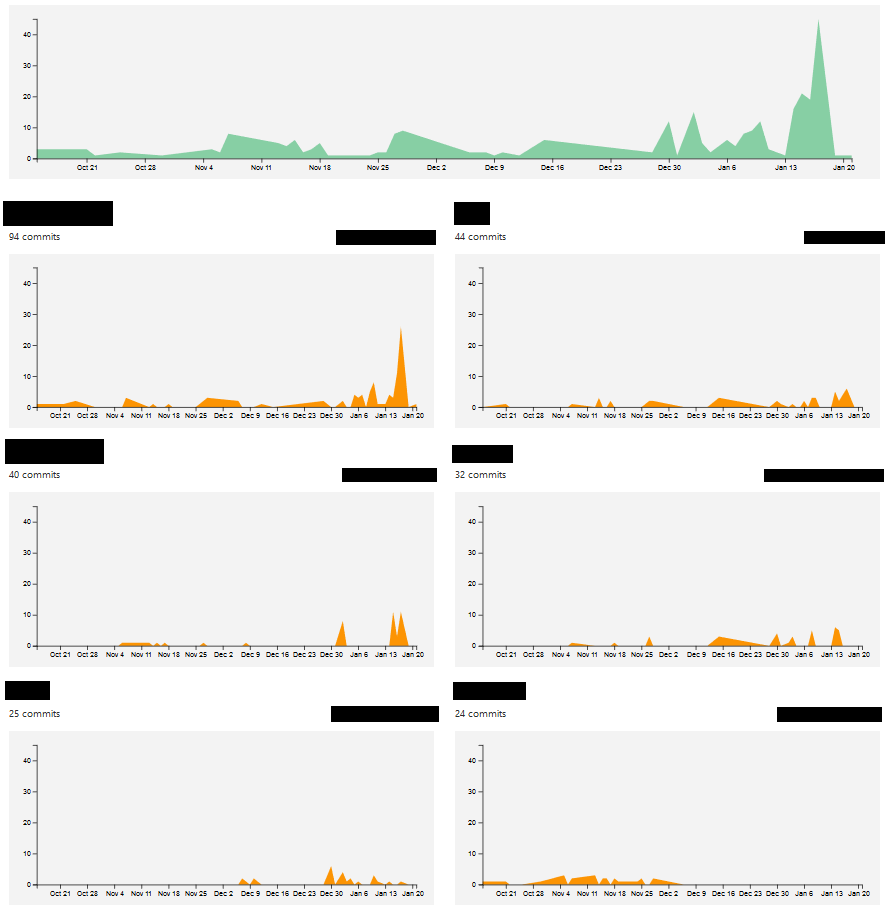
\includegraphics[scale=0.4]{slike/aktivnost.PNG}
			\centering
			\caption{Primjer slike s potpisom}
			\label{fig:promjene}
		\end{figure}
		
		\begin{figure}[H]
			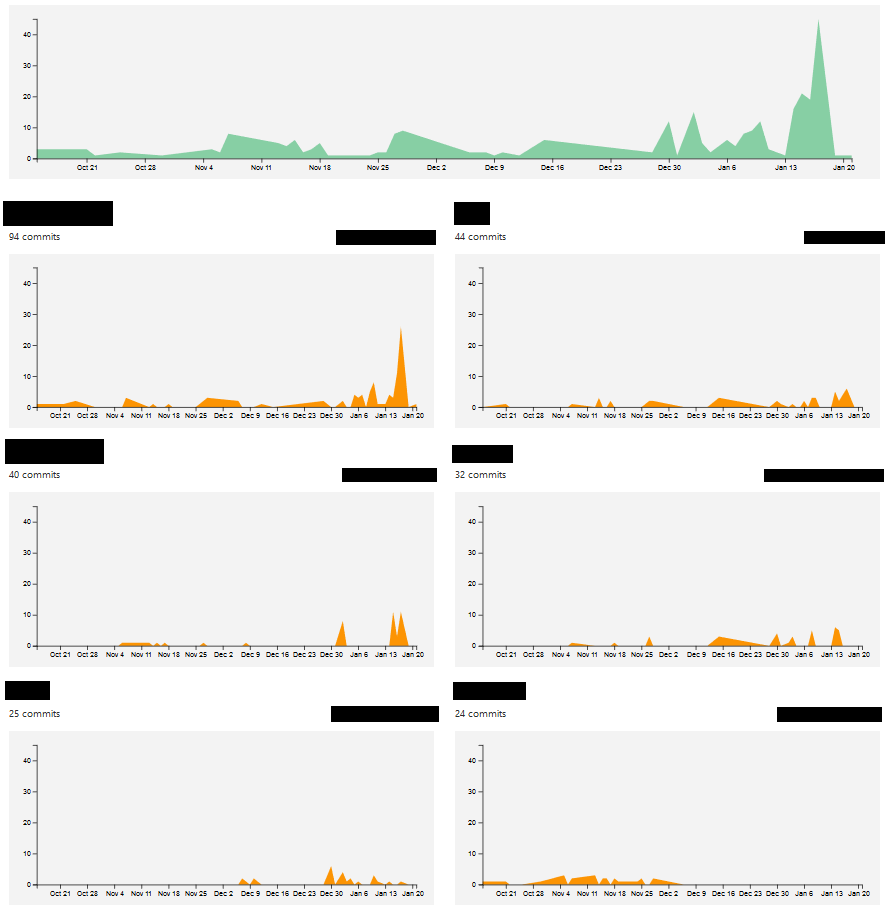
\includegraphics[width=\linewidth]{slike/aktivnost.PNG}
			\caption{Primjer slike s potpisom 2}
			\label{fig:promjene2}
		\end{figure}
		
		
		
		\eject
		
	